\chapter{Experimental Setup}
\section{CERN}
International laboratory in Europe, founded 1959?, maybe little significant history.  

\section{LHC}
All the good stats on the LHC: circumference, (place,) dipole design, magnets, magnetic field.  Design energy and luminosity.  

\section{CMS}
Important stats on CMS: height, weight, etc.  

Figure: Event display, Fig. \ref{fig:EventDisplay}

 \begin{figure}[htb]
  \begin{center}
    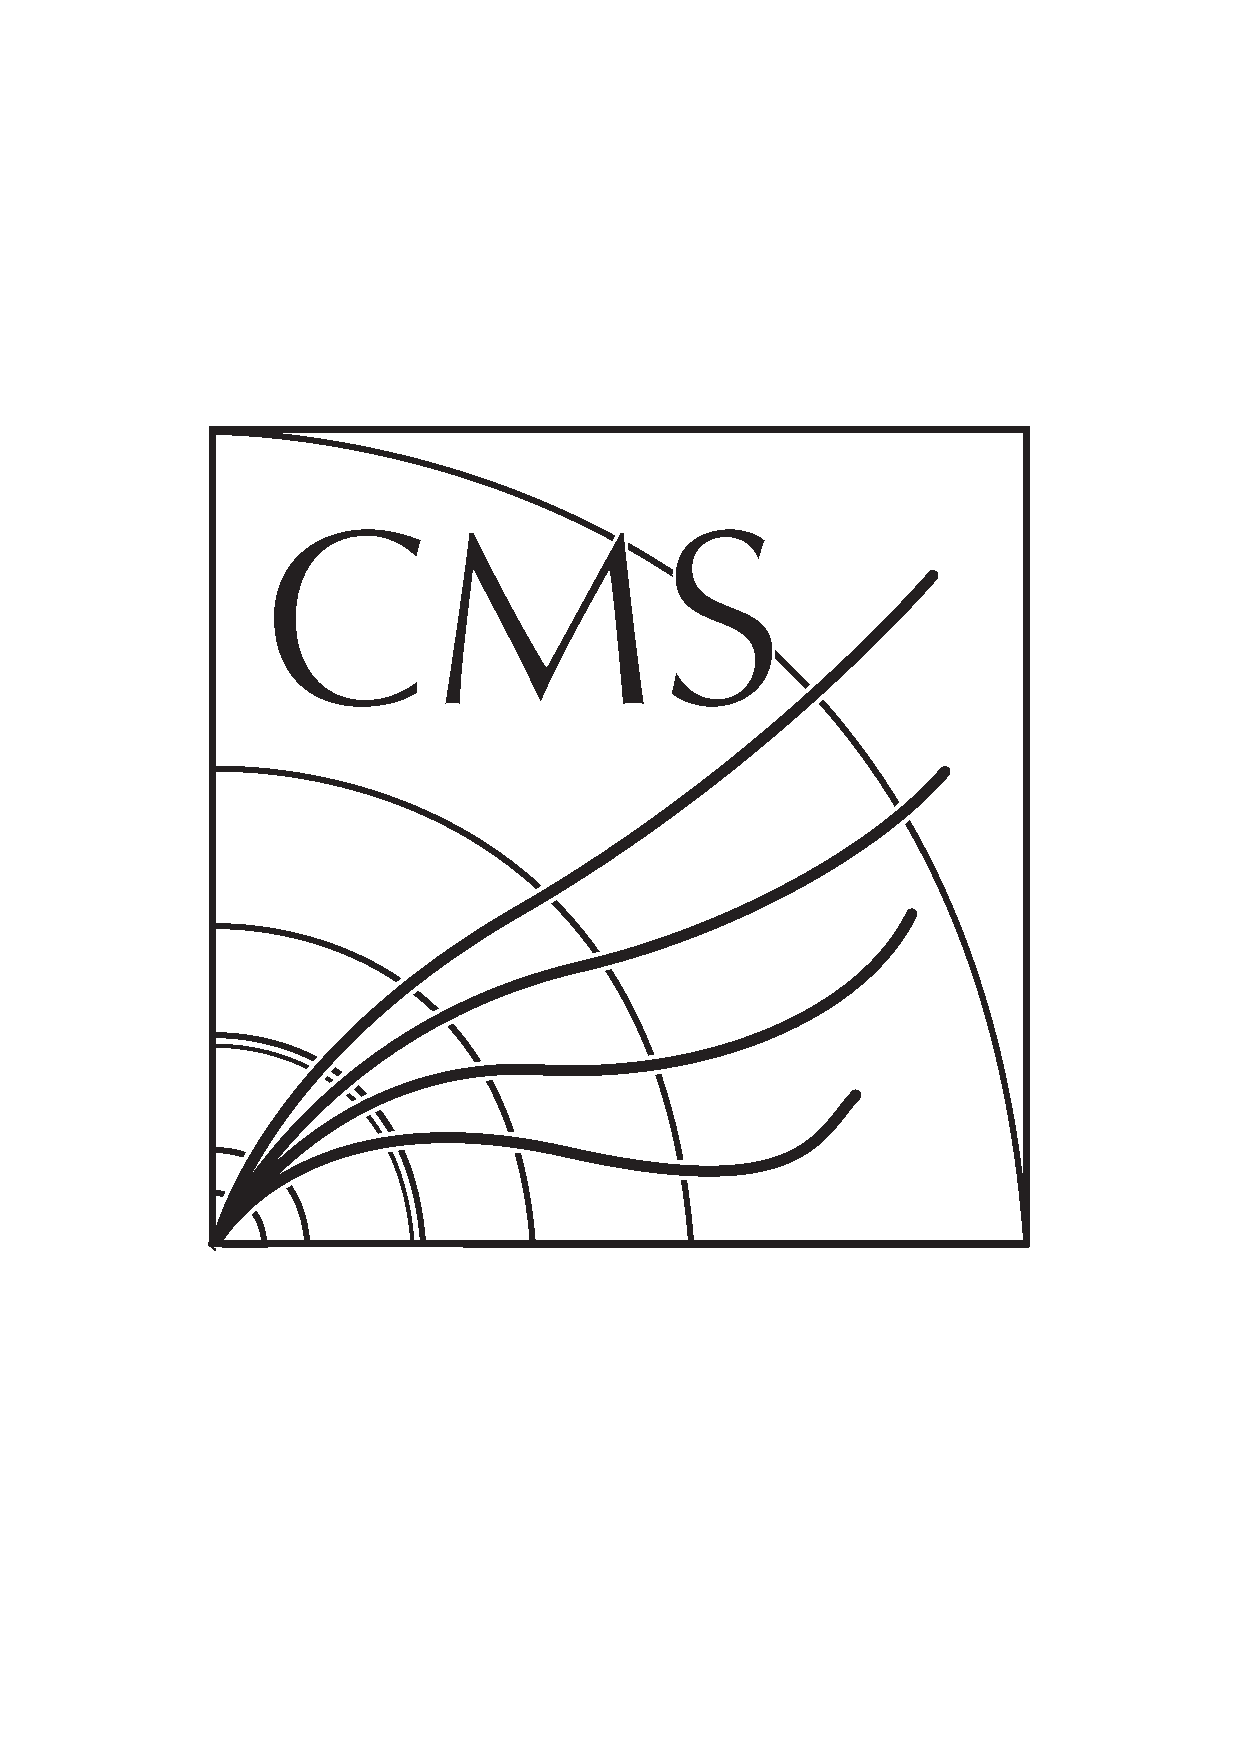
\includegraphics[width=360pt]{CMS-BW.pdf}
  \end{center}
  \caption[Three-dimensional display of a \Zee event in the CMS detector]{Three-dimensional display of a \Zee event in the CMS detector.}
  \label{fig:EventDisplay}
 \end{figure}

\subsection{Detection of Particle Interactions}
\subsection{Coordinate System}
\subsection{Magnet}
\subsection{Luminosity}
Figure: Luminosity plot, Fig. \ref{fig:LuminosityVsTime}

 \begin{figure}[htb]
  \begin{center}
    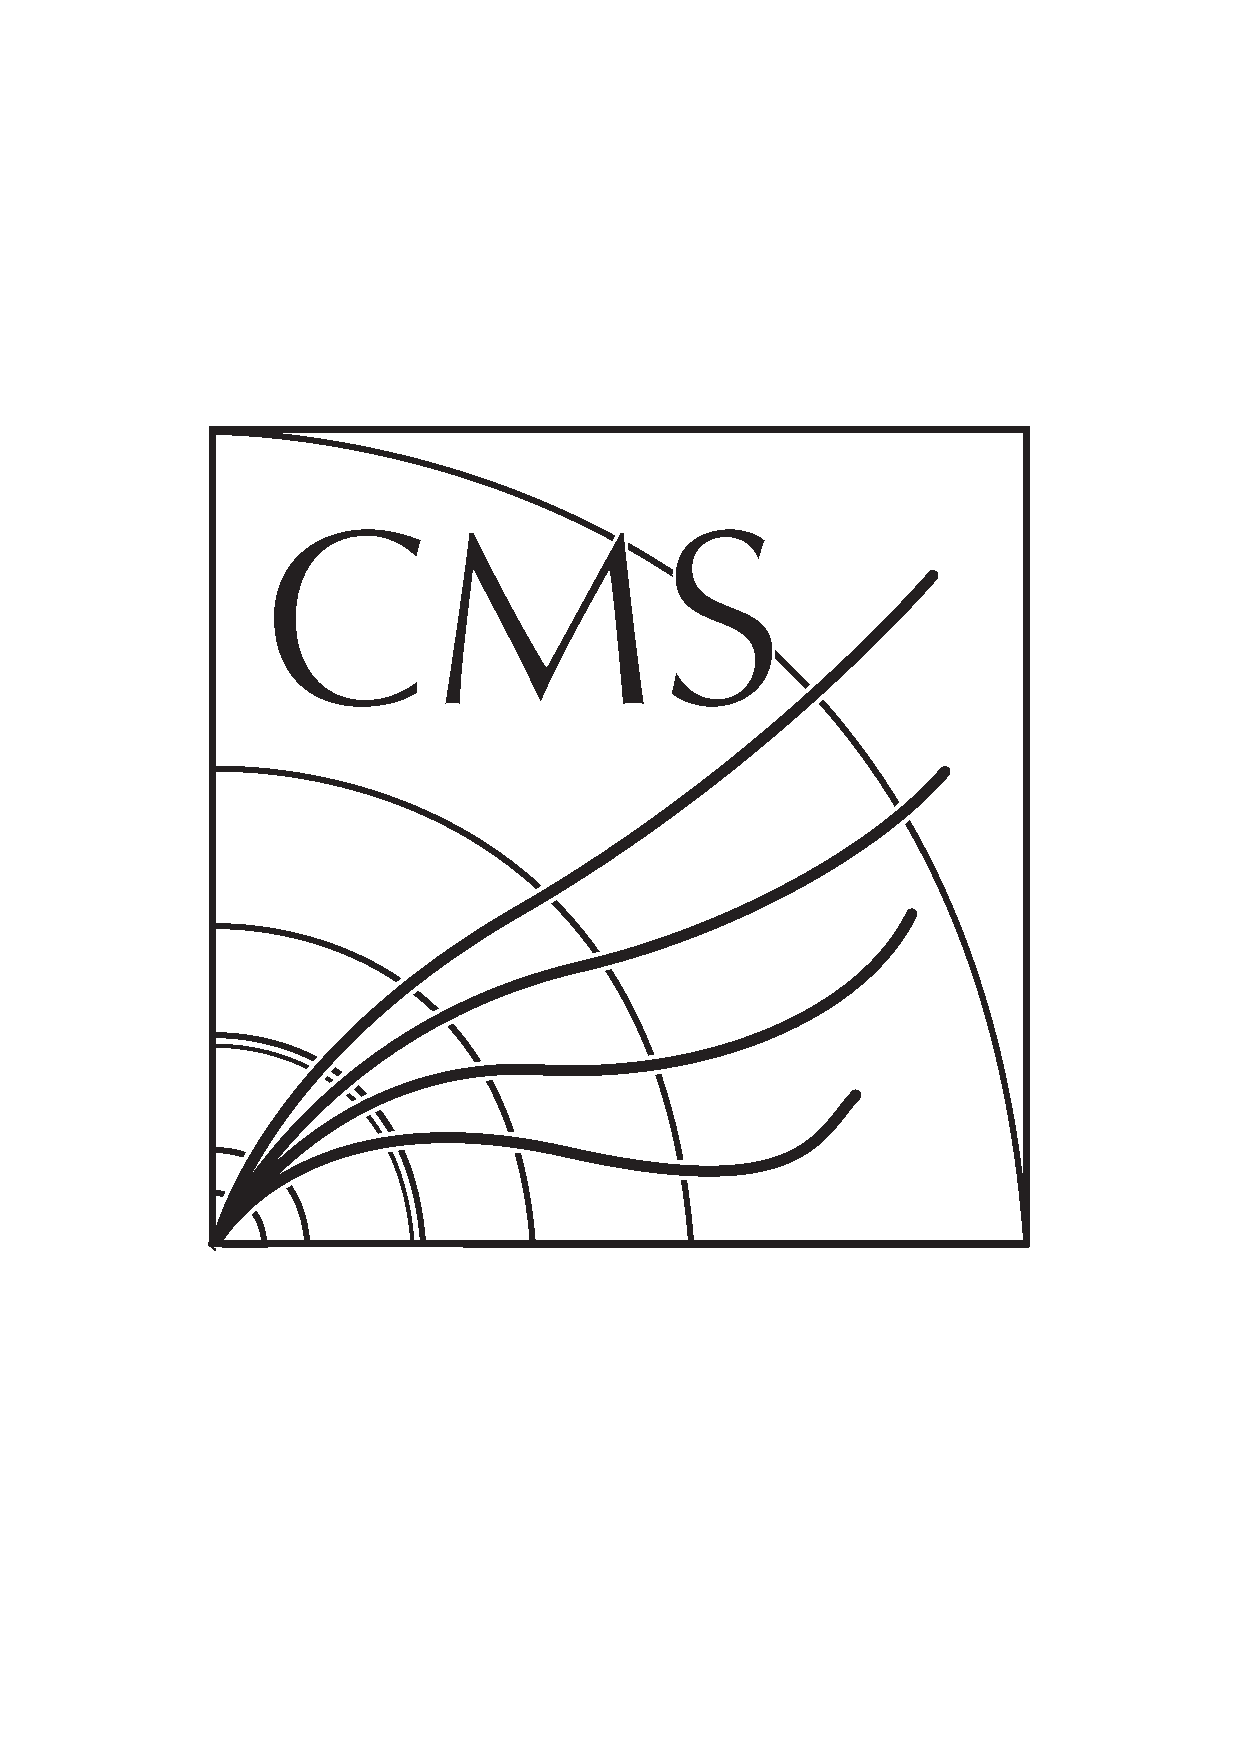
\includegraphics[width=360pt]{CMS-BW.pdf}
  \end{center}
  \caption[Luminosity as a function of time]{Luminosity as a function of time.}
  \label{fig:LuminosityVsTime}
 \end{figure}

\subsection{Calorimeters}
\subsubsection{ECAL}
\subsubsection{HCAL}
\subsection{Muon Systems}
\subsection{Tracker}
\subsection{Pixels}
\subsection{Trigger}
\subsubsection{Level-1 Trigger}
General L1 information, specific electron algorithms in online selection section.  
\subsubsection{High-Level Trigger}
General HLT information, specific electron algorithms in online selection section.  
